\section{Hidden Markov Model}

\subsection{Markov Chain}
「コイントスして,表なら左へ一歩,裏なら右へ一歩」を延々と繰り返すという最も基本的な確率過程のことを\textbf{ランダムウォーク(酔歩)}という.
左右の確率を変えたり前後左右へ動くようにしたりと,バリエーションはいろいろ考えられるが,ここでは単純に一次元で左右等確率の設定とする.
形式的に書くと,$+1$か$-1$かが半々の確率で出るi.i.d\footnote{独立同一分布(independent and indentically distributed; i.i.d)}な確率変数たち$Z_{1}, Z_{2}, Z_{3},...$を使って,
\begin{equation}
X_{0}=0, \quad X_{t} = X_{t-1} + Z_{t} \ (t=1,2,...) \label{eq:ranwark}
\end{equation}
と表される$X_{t}$のことである\cite{probability_statistics_for_programming}.

ランダムウォークの場合,
\begin{equation}
P(X_{t+1} = x_{t+1} | X_{t} = x_{t},X_{t-1} = x_{t-1}, ... , X_{0} = x_{0}) = P(X_{t+1}=x_{t+1}|X_{t} = x_{t}) \label{eq:markov}
\end{equation}
が成り立つ.
つまり,未来の状態は今の状態だけから定まり,過去の履歴(どこからどんな経路をたどって今の状態にたどりついたか)には無関係であった.
現在の状態が一時点前の状態に依存して確率的に決まるような特性を\textbf{マルコフ性(Markov property)}という.
そしてこのような確率過程を\textbf{マルコフ過程(Markov process)}という.
その中でも特に,$X_{t}$がとり得る値が有限とおりなものを\textbf{マルコフ連鎖(Markov chain)}と呼ぶ.

マルコフモデルは複数の状態を持ち,ある状態から別の状態(元の状態も含む)へ一定の確率で遷移する.
この確率を\textbf{遷移確率(transition probability)}という.
また,現在の状態に依存した一定の確率で特定の\textbf{出力記号(output symbol)}を出力する.
この確率を\textbf{出力確率(output probability)}という\cite{probability_statistics_for_programming}.

\newpage

\subsection{モデル概要}
例として,2種類のサイコロ(状態)$\omega_{1}$,$\omega_{2}$を投げて出た目を観測する場合を考える.
ここではサイコロの目(出力記号)として奇数と偶数の2種類を考える.

初期確率$\bm{\pi}$,遷移確率行列$\bm{A}$,出力確率行列$\bm{B}$が以下のように与えられたとする.

\begin{equation}
\bm{\pi} = \hspace{1zw}
\bordermatrix{
	& \omega_{1} & \omega_{2} \cr
	& 0.2 & 0.8
}
\end{equation}

\begin{equation}
\bm{A} = \hspace{1zw}
\bordermatrix{
						 & \omega_{1} & \omega_{2}  \cr
	\omega_{1} & 0.7 & 0.3  \cr
	\omega_{2} & 0.6 & 0.4  \cr
}
\end{equation}

\begin{equation}
\bm{B} = \hspace{1zw}
\bordermatrix{
						 & 奇数 & 偶数  \cr
	\omega_{1} & 0.5 & 0.5  \cr
	\omega_{2} & 0.9 & 0.1  \cr
}
\end{equation}

行列$\bm{A}$と初期確率$\bm{\pi}$により,遷移確率$\pi_{i}$,$a_{ij}$を反映した状態遷移系列が得られ,行列$\bm{B}$により,各状態からの出力確率$b_{jk}$を反映した出力記号系列が得られる.
状態遷移と記号の出力の様子を図\ref{fig:markov:markovmodel}(\subref{fig:markov:markovmodel1})に示す.

時刻$t$における状態を$s_{t}$,出力記号を$x_{t}$として,グラフィカルモデルで表したものを図\ref{fig:markov:markovmodel}(\subref{fig:markov:markovmodel2})に示す.
このモデルにおいて,状態系列と出力系列の両方を観測することができるものを\textbf{マルコフモデル(Markov Model)},
状態系列が観測できず出力系列のみを観測することができるものを\textbf{隠れマルコフモデル(Hidden Markov Model; HMM)}という.

\begin{figure}[htb]
	\centering
	\begin{minipage}[t]{.49\hsize}
		\centering
		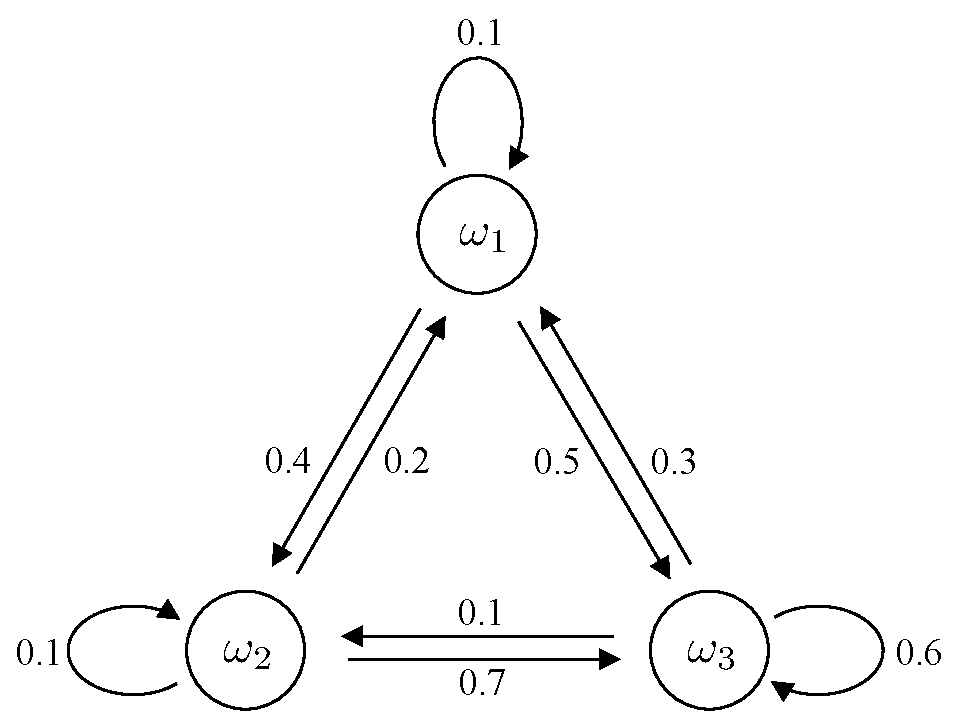
\includegraphics[width=\hsize, bb=0 0 461 344]{./fig/hidden_markov_model/markov_model.pdf}
		\subcaption{状態遷移図}
		\label{fig:markov:markovmodel1}
	\end{minipage}
	\begin{minipage}[t]{.5\hsize}
		\centering
		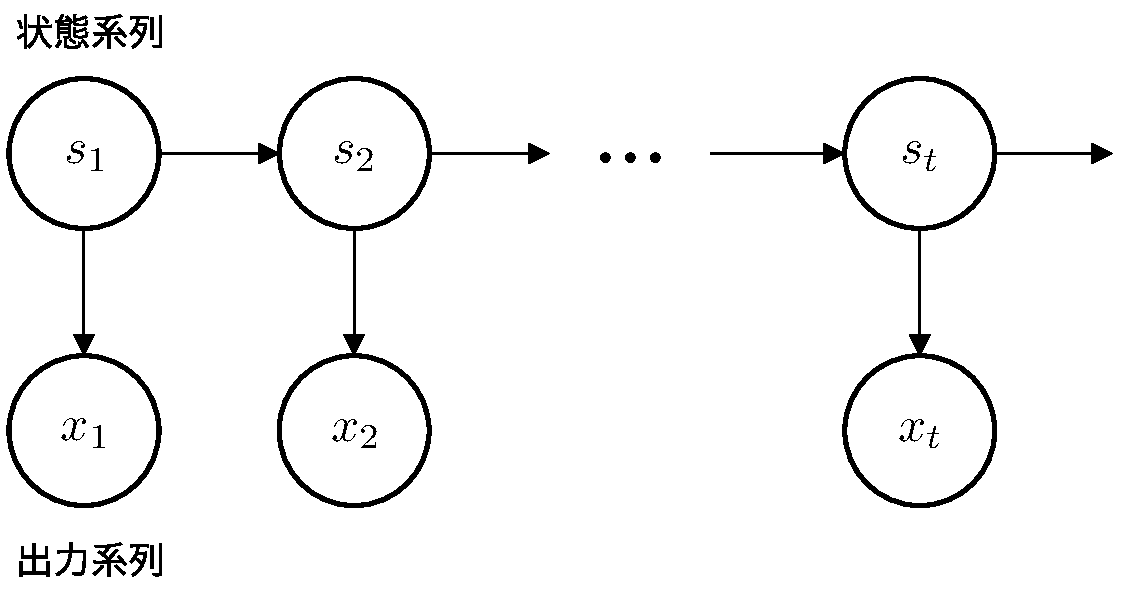
\includegraphics[width=\hsize, bb=0 0 551 289]{./fig/hidden_markov_model/markov_graph.pdf}
		\subcaption{状態空間モデル}
		\label{fig:markov:markovmodel2}
	\end{minipage}
	\caption{マルコフモデル}
	\label{fig:markov:markovmodel}
\end{figure}

\newpage
\subsection{確率モデル}

\begin{myframe}{Notation of HMM}
	\begin{tabular}{ll}
		$N$ & :状態数 \\
		$M$ & :出力記号の数 \\
		$s_{t} \in \{\omega_{1}, \omega_{2},..., \omega_{N}\}$ & :時点$t$での状態 \\
		$x_{t} \in \{v_{1}, v_{2},..., v_{M}\}$ & :時点$t$での観測結果(出力記号) \\
		$\mathbf{s} = s_{1}s_{2}\cdots s_{t} \cdots s_{T}$ & :状態系列 \\
		$\mathbf{x} = x_{1}x_{2}\cdots x_{t} \cdots x_{T}$ & :観測記号系列 \\
		$\pi_{i}$ & :初期状態($t=1$)が$\omega_{i}$である確率 $P(s_{1} = \omega_{i})$ \\
		$a_{ij},a(\omega_{i}, \omega_{j})$ & :状態$\omega_{i}$から状態$\omega_{j}$への遷移確率 $P(s_{t} = \omega_{j} | s_{t-1} = \omega_{i})$ \\
		$b_{jk},b(\omega_{j}, v_{k})$ & :状態$\omega_{j}$で$v_{k}$を出力する確率 $P(x_{t} = v_{k} | s_{t} = \omega_{j})$\\
		$\bm{\pi}=(\pi_{1}, \pi_{2}, ..., \pi_{N})$ & :$\pi_{i}$を成分としてもつ$N$次元のベクトル \\
		$\bm{A}$ & :$a_{ij}$を($i,j$)成分としてもつ$N \times N$の行列 \\
		$\bm{B}$ & :$b_{jk}$を($j,k$)成分としてもつ$M \times M$の行列 \\
	\end{tabular}
\end{myframe}

\subsubsection{状態遷移確率}
\begin{equation}
	a_{ij} = P(s_{t} = \omega_{j} | s_{t-1} = \omega_{i})
\end{equation}

\subsubsection{出力確率}
\begin{equation}
	b_{jk} = P(x_{t} = v_{k} | s_{t} = \omega_{j})
\end{equation}

\subsection{パラメータ推定}

隠れマルコフモデルでは,最尤推定を用いて観測系列よりパラメータ推定を行う.
推定すべきパラメータ$\bm{\pi},\bm{A},\bm{B}$をまとめて
\begin{equation}
\bm{\theta} = (\bm{\pi},\bm{A},\bm{B})
\end{equation}
とする.

最尤推定により最適なパラメータ$\bm{\theta}$を求めることは,$P(\mathbf{x}; \bm{\theta})$を$\bm{\theta}$に関して最大化することである.
そのためにはEMアルゴリズムを適用し,Q関数を最大化すれば良い.

\begin{equation}
Q(\bm{\theta}^{0}, \bm{\theta}) = \sum_{\mathbf{s}} P(\mathbf{s} | \mathbf{x}; \bm{\theta}^{0}) \log P(\mathbf{x}, \mathbf{s}; \bm{\theta}) \label{eq:Qfunc}
\end{equation}

ここで,$\bm{\theta}$は$\bm{\theta}^{0}$を更新した結果得られる新しいパラメータである.Q関数を最大化するには,パラメータを繰り返し更新すればよい.

式(\ref{eq:Qfunc})を式変形すると,
\begin{align}
Q(\bm{\theta}^{0}, \bm{\theta}) & = \sum_{\mathbf{s}} P(\mathbf{s} | \mathbf{x}; \bm{\theta}^{0}) \log P(s_{1}) + \sum_{\mathbf{s}} P(\mathbf{s} | \mathbf{x}; \bm{\theta}^{0}) \sum_{t=1}^{n-1} \log a(s_{t}, s_{t+1}) + \sum_{\mathbf{s}} P(\mathbf{s} | \mathbf{x}; \bm{\theta}^{0}) \sum_{t=1}^{n}\log b(s_{t}, x_{t}) \\
& = Q(\bm{\theta}^{0}, \bm{\pi}) + Q(\bm{\theta}^{0}, \bm{A}) + Q(\bm{\theta}^{0}, \bm{B})
\end{align}
が得られる.ここで,
\begin{align}
Q(\bm{\theta}^{0}, \bm{\pi}) & \overset{\mathrm{def}}{=} \sum_{\mathbf{s}} P(\mathbf{s} | \mathbf{x}; \bm{\theta}^{0}) \log P(s_{1}) \\
Q(\bm{\theta}^{0}, \bm{A}) & \overset{\mathrm{def}}{=} \sum_{\mathbf{s}} P(\mathbf{s} | \mathbf{x}; \bm{\theta}^{0}) \sum_{t=1}^{n-1} \log a(s_{t}, s_{t+1}) \\
Q(\bm{\theta}^{0}, \bm{B}) & \overset{\mathrm{def}}{=} \sum_{\mathbf{s}} P(\mathbf{s} | \mathbf{x}; \bm{\theta}^{0}) \sum_{t=1}^{n}\log b(s_{t}, x_{t}) \label{eq:Q_B}
\end{align}
と定義した.上の3式は,それぞれパラメータ$\bm{\pi},\bm{A},\bm{B}$のみを含む.
したがって,$Q(\bm{\theta}^{0}, \bm{\theta})$を$\bm{\theta}$について最大化するには,$Q(\bm{\theta}^{0}, \bm{\pi}),Q(\bm{\theta}^{0}, \bm{A}),Q(\bm{\theta}^{0}, \bm{B})$を,
それぞれパラメータ$\bm{\pi},\bm{A},\bm{B}$について最大化すればよい.
ここで,$\bm{\theta}^{0}$は更新前のパラメータであるので,最大化に当たっては定数とみなしてよい.

本手法はEMアルゴリズムに則っているので,パラメータ$\bm{\pi},\bm{A},\bm{B}$を適当な初期値に設定し,各パラメータの更新式を反復的に計算することにより,より良い推定値が得られることが保証されている.
この計算方法は\textbf{バウム・ウェルチアルゴリズム(Baum-Welch algorithm)}と呼ばれている\cite{zokupata, levinson1983introduction}.
ただし,得られる解は最適解である保証はなく,一般的には局所的最適解である.

式の導出など詳しい情報は,私の過去のゼミの資料や,参考文献\cite{zokupata}8章,参考文献\cite{bishop:2006:PRML}13章2節を参照してほしい.
